The Volume/Balance module (\verb=Vol_Bal=) acts as the hub for processing incoming digital audio signals, forwarded from WM8731 via the \verb=Snd_Driver= module. As such, \verb=Vol_Bal= also keeps internal registers in the module \verb=Current_Vol_Bal= that holds volume (4-bit unsigned) and balance levels (4-bit signed), as well as a mute signal (std\_logic). These registers update via the one-hot coded input signal \verb=kb_input= applied by the \verb=Keyboard= module. Consequently, the values they hold are not only used as signals (\verb=i_volume_lvl=, \verb=i_balance_lvl=, \verb=i_mute=) for the internal submodule that process the \verb=LADC= and \verb=RADC= inputs, but also as module outputs connected to the \verb=VGA_Driver= so that they can be rendered on the screen.

\begin{figure}[H]
  \centering
  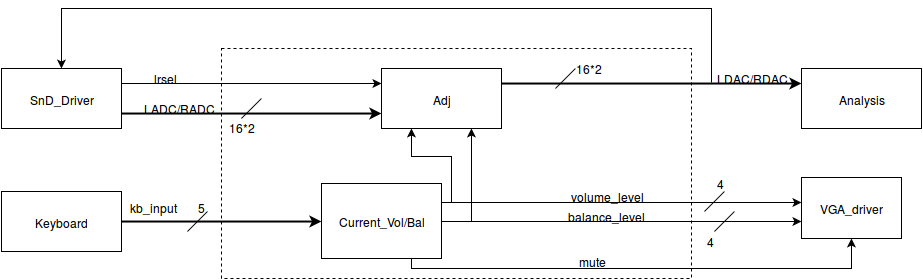
\includegraphics[width=16cm]{volbal}
  \caption{An overview of the \texttt{Vol\_Bal} module's internal workings.}
  \label{fig:vol_bal}
\end{figure}

The main function of the Volume/Balance module is to make requested adjustments to incoming values \verb=LADC= and \verb=RADC=, which represent measured amplitudes of the sound signal at distinct times. The sound will first be adjusted for volume using the function:

$$A_{adj} = A_{in} \cdot (1/\sqrt{2})^n$$

Following that, we scale the volume-adjusted amplitude linearly, accounting for balance:

$$A_{l\_out} = \frac{5 - m}{5} \cdot A_{l\_adj}\qquad,\ A_{l\_out} = A_{l\_adj}\ for\ m < 0$$
$$A_{r\_out} = \frac{5 - |m|}{5} \cdot A_{r\_adj}\qquad,\ A_{r\_out} = A_{r\_adj}\ for\ m > 0$$


In the functions above, $A$ is the amplitude, $n$ the volume level and $m$ the balance. \verb=lrsel= is used as a control signal for selecting the channel and the correct function for balance scaling. Resulting outputs \verb=LDAC= and \verb=RDAC= are forwarded to \verb=Snd_Driver= and to one instance of the \verb=Analysis= modules.

Ultimately, the user have the ability to digitally adjust the input sound by decreasing the volume in 3 dB decrements, down to -30 dB, and also to regulate balance bias by linearly scaling outputs on a single left or right audio channel. There is also a mute function which is conveyed by \verb=kb_input=. When active, the register driving the \verb=mute= signal essentially zeroes any $A_{out}$ values on the \verb=LDAC/RDAC= outputs.


